\documentclass[12pt, openany]{report}
\usepackage[utf8]{inputenc}
\usepackage[T1]{fontenc}
\usepackage{amsmath,amsfonts,amssymb}
\usepackage{amssymb}
\usepackage{multicol}
\usepackage[a4paper,left=2.5cm,right=2.5cm,top=2.5cm,bottom=2.5cm]{geometry}
\usepackage[english]{babel}
\usepackage{libertine}
\usepackage{graphicx}
\usepackage{wrapfig}
\usepackage{algorithm}
\usepackage{algpseudocode}
\usepackage{float}
\usepackage{enumitem}
\usepackage{pythonhighlight}
\usepackage[]{titletoc}
\usepackage{empheq}
\usepackage{titlesec}
\usepackage{mathpazo}
\usepackage{xfrac}
\usepackage{textcomp}
\usepackage{mathtools}
\usepackage{caption}
\usepackage{tabularray}
\usepackage{subcaption}
\usepackage[bottom]{footmisc}
\usepackage{pdfpages}
\usepackage{tabularx}
\usepackage {tikz}
\usetikzlibrary{positioning}
\usepackage{amsthm}
\usepackage[skins]{tcolorbox}
\titleformat{\chapter}[display]
  {\normalfont\bfseries}{}{0pt}{\Huge}
\usepackage{hyperref}
\newcommand{\hsp}{\hspace{20pt}}
\newcommand{\HRule}{\rule{\linewidth}{0.5mm}}
\newcommand{\R}{\mathbb{R}}
\newcommand{\C}{\mathbb{C}}
\newcommand{\E}{\mathbb{E}}
\newcommand{\J}{\mathbf{J}}
\newcommand{\He}{\mathbf{H}}
\theoremstyle{definition}
\newtheorem{thm}{Theorem}[chapter]
\newtheorem{definition}[thm]{Definition}
\newtheorem{lem}[thm]{Lemma}

\hbadness=100000
\begin{document}
\begin{titlepage}
    \begin{sffamily}
    \begin{center}
        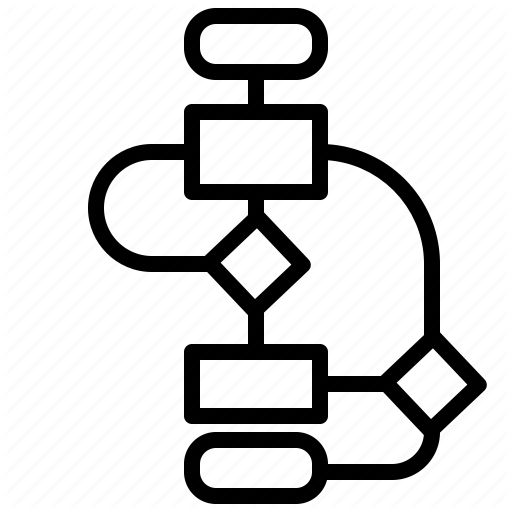
\includegraphics[scale=0.3]{img/page_de_garde.jpg} \\[1cm]
        \HRule \\[0.4cm]
        { \huge \bfseries LINMA2472 - Algorithm in data science \\[0.4cm] }
    
        \HRule \\[1.5cm]
        \textsc{\LARGE Simon Desmidt}\\[1cm]
        \vfill
        \vspace{2cm}
        {\large Academic year 2025-2026 - Q1}
        \vspace{0.4cm}
         
        
\includegraphics[width=0.15\textwidth]{img/epl.png}
        
        UCLouvain\\
    
    \end{center}
    \end{sffamily}
\end{titlepage}

\setcounter{tocdepth}{1}
\tableofcontents
\chapter{Automatic differentiation}
The Automatic differentiation is an algorithmic technique to compute automatically the derivative (gradient) of a function defined in a computer program. Unlike symbolic differentiation (done by hand) and numerical  differentiation (finite difference approximation), automatic differentiation exploits the fact that every function can be decomposed into a sequence of elementary operations (addition, multiplication, sine, exponential, etc.) and so that we can apply the chain rule to compute the derivative of the whole function. Thus we can compute the gradient of a function exactly and efficiently.\\ 
Automatic differentiation is widely used in machine learning because for the neural networks, we need to compute the gradient of a loss function with respect to the parameters of the model (weights and biases) to update them during the training process and it would be difficult to compute this manually for each node.\\
\section{Chain rule}
There is two ways to apply the chain rule to compute the gradient of a function: forward differentiation and backward differentiation. Suppose that we have a composition of $m$ functions. The chain rule gives us:
\begin{equation}
  f'(x) = f_m'(f_{m-1}(f_{m-2}(...f_1(x)...))) \cdot ... \cdot f_2'(f_1(x)) \cdot f_1'(x)
\end{equation}
Let's define:
\begin{equation}
  \begin{cases}
    s_0 &= x \\
    s_k &= f_k(s_{k-1})
  \end{cases}
\end{equation}
We thus get:
\begin{equation}
  f'(x) = f'_m(s_{m-1}) \cdot ...
  \cdot f'_2(s_1) \cdot f'_1(s_0)
\end{equation}
Based on this, we can define the forward and backward differentiation algorithms.
\section{Forward differentiation}
Also called forward mode, this algorithm consists in propagating forward the derivative and the values at the same time. It can be represented by this graph where the blue part represents the values and the green part the derivatives:
\begin{figure}[H]
    \centering
    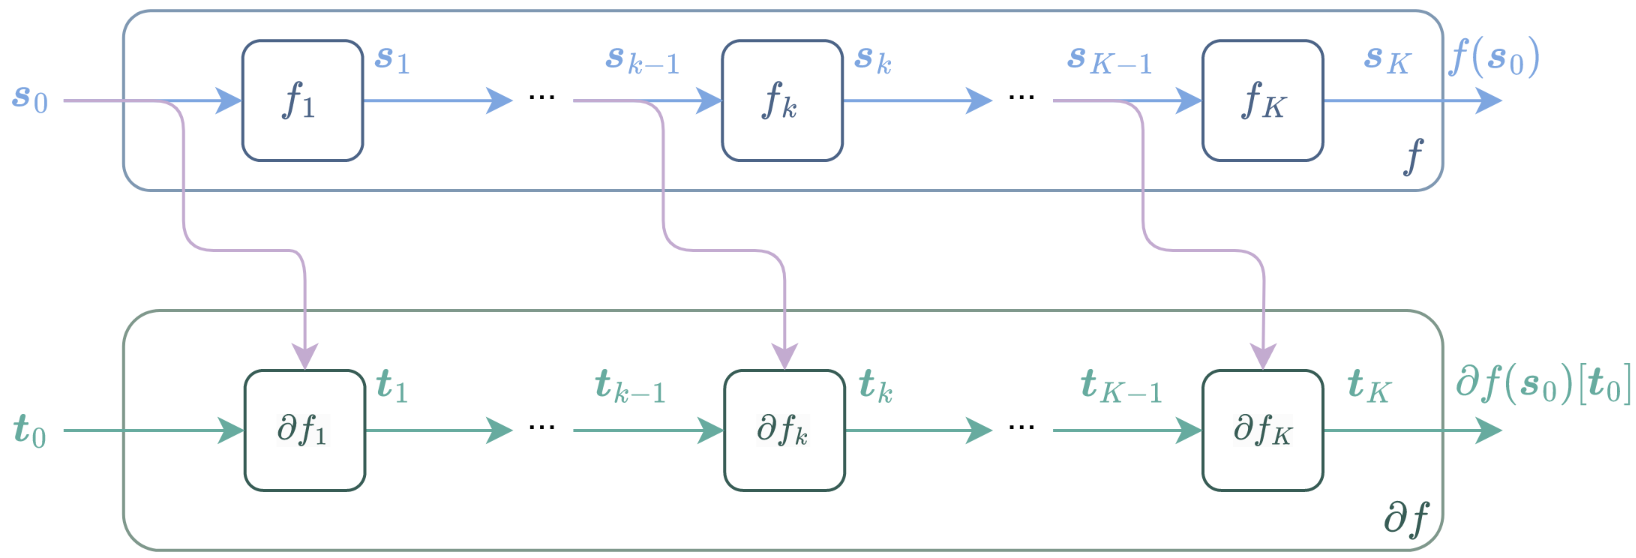
\includegraphics[width=\textwidth]{img/forward_diff.png}
    \caption{Forward differentiation}
    \label{fig:forward_diff}
\end{figure}
And it can be computed with the following recurrence relation:
\begin{equation}
  \begin{cases}
    t_0 &= 1 \\
    t_k &= f'_k(s_{k-1}) \cdot t_{k-1}\\
  \end{cases}
\end{equation}
It is simple to implement and very efficient for functions with a small number of input variables. However, it becomes inefficient for functions with a large number of input variables because we need to compute the derivative for each input variable separately. So in practice for neural networks where we have a large number of input variables (weights and biases), we use the backward differentiation.
\section{Backward differentiation}
Also called backward mode, this algorithm consists in propagating the derivative backward and the values forward at the same time. It can be represented by this graph where the blue part represents the values and the orange part the derivatives:
\begin{figure}[H]
    \centering
    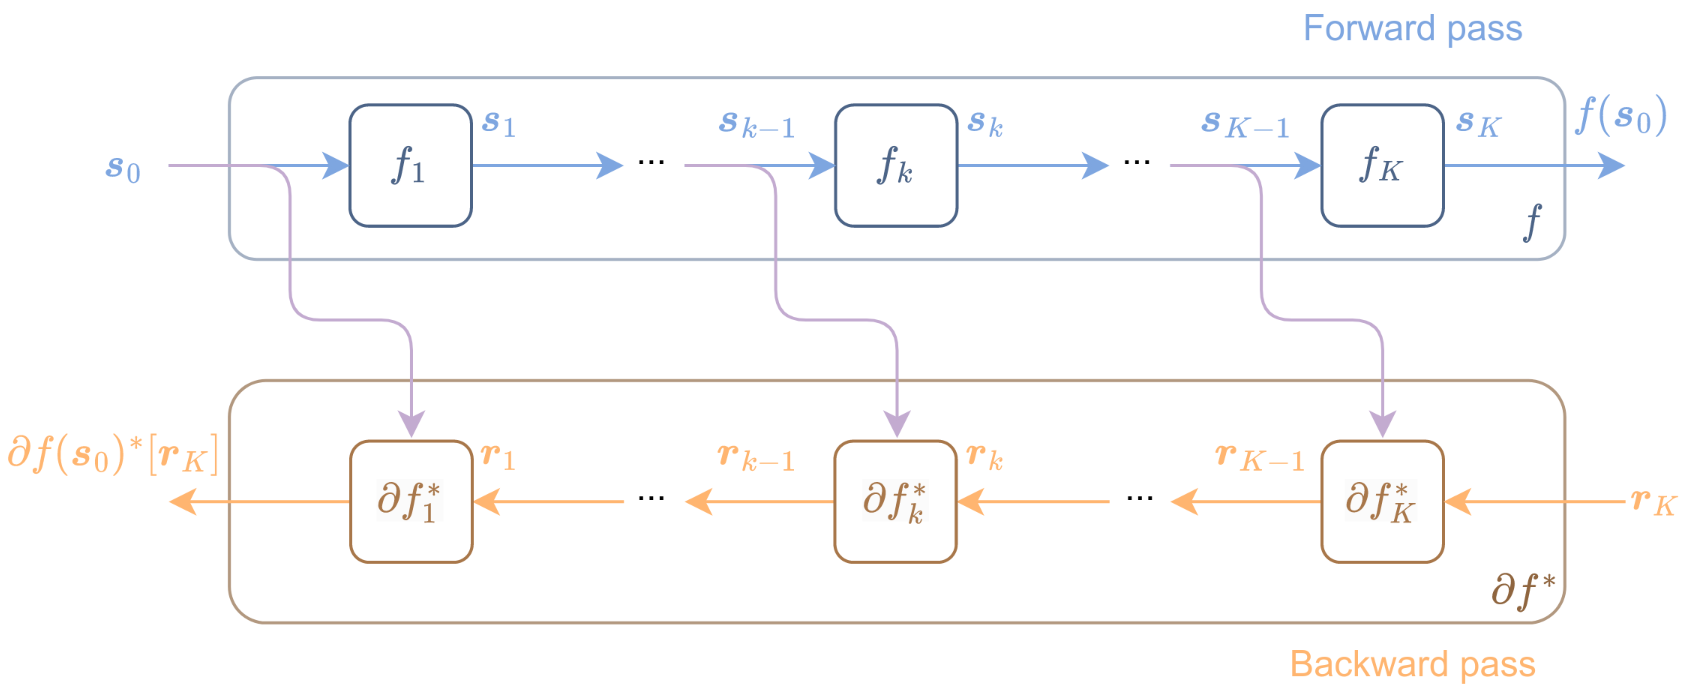
\includegraphics[width=\textwidth]{img/backward_diff.png}
    \caption{Backward differentiation}
    \label{fig:backward_diff}
\end{figure}
The idea is to compute all the intermediate values $s_k$ in a forward pass and then compute the derivatives $r_k$ based on the output in a backward pass. It can be computed with the following recurrence relation:
\begin{equation}
  \begin{cases}
    r_m &= 1 \\
    r_k &= r_{k+1} \cdot f'_{k+1}(s_{k})\\
  \end{cases}
\end{equation}
This method is more complex to implement but it is very efficient for functions with a large number of input variables and a small number of output variables typically 1, the loss function.
\section{Computational graph and multivariate differentiation}
\subsection{Computational graph}  
To represent the computation of a function, we can use a computational graph. It is a directed acyclic graph where the nodes represent the operations and the edges represent the variables. For example, consider the function with $f_1(x)=x=s_1$ and $f_2(x)=x^2=s_2$:
\begin{equation}
  f_3(s_1,s_2) = s_1 + s_2 = x + x^2
\end{equation}
The computational graph is:\\
\begin{center}
  \begin{tikzpicture}[
    roundnode/.style={circle, draw=green!60, fill=green!5, very thick, minimum size=7mm},]
    %Nodes
    \node[roundnode] (x1) {$s_1=x$};
    \node[roundnode] (square) [right=of x1] {$f_2=x^2$};
    \node[roundnode] (sum) [right=of square] {$f_3=f_2+s_1$};
    
    % %Lines
    \draw[->] (x1.north) .. controls +(up:7mm) and +(up:7mm).. (sum.north);
    \draw[->] (x1.east) -- (square.west);
    \draw[->] (square.east) -- (sum.west);
  \end{tikzpicture}
\end{center}
\subsection{Multivariate differentiation}
Let's consider the function of the computational graph above:
\begin{equation}
  f_3(f_1(x),f_2(x)) = s_3 = f_1(x) + f_2(x) = s_1 + s_2 = x + x^2 
\end{equation}
following the chain rule, we have:
\begin{equation}
  f'_3(x) = \frac{\partial f_3}{\partial s_1} \frac{\partial s_1}{\partial x} + \frac{\partial f_3}{\partial s_2} \frac{\partial s_2}{\partial x}
\end{equation}
For the forward automatic differentiation, we work the same way as before, we propagate the values and the derivatives forward. But when we have a node with multiple inputs, we need to use formula derivated from the chain rule. For the function $f_3$ that we want to evaluate in $x=3$, we will have:
\begin{equation}
	\begin{cases}
		t_0 &= 1 \\
		t_1 &= f'_1(x) \vert_{x=3} \cdot t_0 = 1\\
		t_2 &= f'_2(x) \vert_{x=3} \cdot t_0 = 6\\
		t_3 &= \frac{\partial f_3}{\partial s_1} \vert_{x=3} \cdot t_1 + \frac{\partial f_3}{\partial s_2} \vert_{x=3} \cdot t_2 = 7\\
	\end{cases}
\end{equation}
For the backward automatic differentiation, first we need to initialize the gradient accumulator to 0.
\begin{equation}
	\frac{\partial s_3}{\partial s_1} = \frac{\partial s_3}{\partial s_2} = \frac{\partial s_3}{\partial x} = 0
\end{equation}
Then we compute the intermediate values in a forward pass:
\begin{equation}
	\begin{aligned}
		\frac{\partial s_3}{\partial s_1} &+= 1 \Rightarrow \frac{\partial s_3}{\partial x} += 1 \cdot 1 \vert_{x=3}\\		
		\frac{\partial s_3}{\partial s_2} &+= 1 \Rightarrow \frac{\partial s_3}{\partial x} += 1 \cdot 2x \vert_{x=3}\\
	\end{aligned}
\end{equation}
Finally we get:
\begin{equation}
	\frac{\partial s_3}{\partial x} = 7
\end{equation}
\section{Jacobian computation}
When doing the forward and backward mode, we compute the Jacobian matrix of the function. 
Using this Jacobian we can do the forward mode like this:
\begin{equation}
  J_f(x) \cdot v \qquad \qquad \text{(JVP)}
\end{equation}
where $v$ is a vector of size $n$ (number of input variables)
and the backward mode like this:
\begin{equation}
  v^T J_f(x) \qquad \qquad \text{(VJP)}
\end{equation}
Consider a function $f:\R^n \rightarrow \R^m$ then computing the full Jacobian requires $n$ forward passes (JVP) or $m$ backward passes (VJP). Therefore,
\begin{itemize}
  \item If $n \ll m$, we use the forward mode because it's faster
  \item If $n \gg m$, we use the backward mode because it's faster
  \item If $n \approx m$, we can use either mode
\end{itemize}
\section{Memory usage}
The forward mode only needs to store the current value and the current derivative, so the memory usage is relatively constant.\\
\begin{figure}[H]
    \centering
    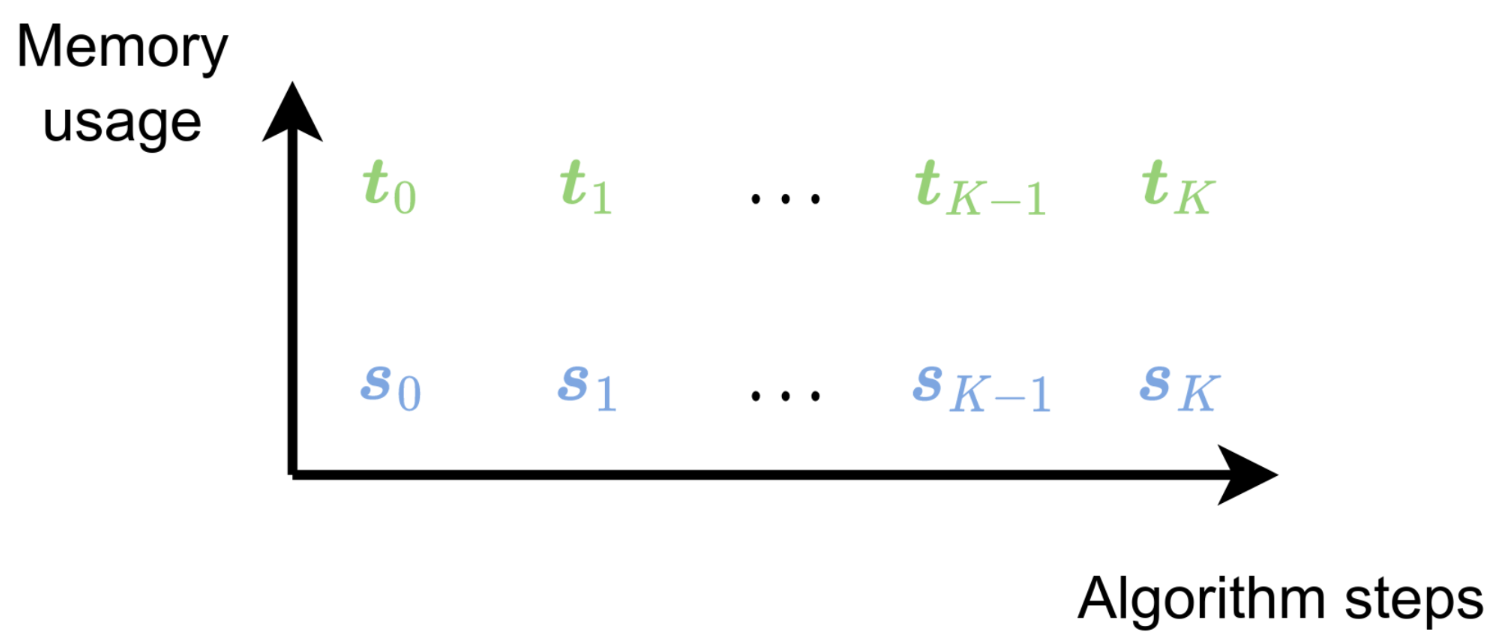
\includegraphics[width=\textwidth]{img/fd_mem.png}
    \caption{Forward mode memory usage}
    \label{fig:fd_mem}
\end{figure}
However, the backward mode needs to store all the intermediate values to compute the derivatives in the backward pass so the memory usage will first increase then reduce when we will start to use the derivatives previously computed.\\
\begin{figure}[H]
    \centering
    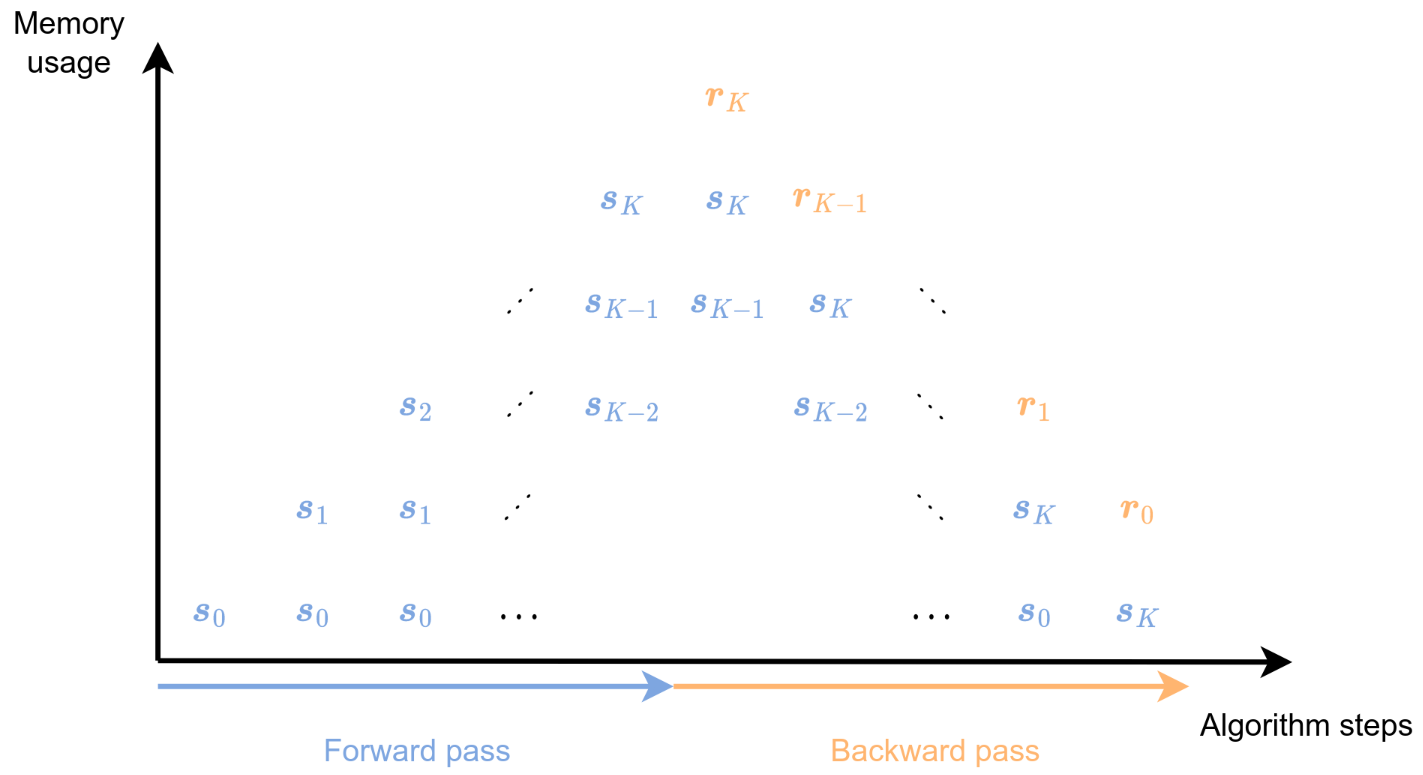
\includegraphics[width=\textwidth]{img/bd_mem.png}
    \caption{Backward mode memory usage}
    \label{fig:bd_mem}
\end{figure}
So the forward mode is more memory efficient than the backward mode. However, this factor may be less significant than the number of operations performed (JVP and VJP).
\section{Second order AD}
And what happens when we take a look at the second order derivative? Remember that we can compute the Hessian $\nabla^2 f(x)$ like this:
\begin{equation}
  (\nabla^2 f(x))_{ij} = \frac{\partial^2 f(x)}{\partial x_i \partial x_j}
\end{equation}
Or like this:
\begin{equation}
  \nabla^2 f(x) = J_{\nabla f}(x)
\end{equation}
We can easily see that with this definition, we can use an AD for the gradient and for the Jacobian to compute the Hessian. And because we can separate these two computations in distinct AD, it means that we are not forced to use the same mode for both. So we can do either forward or backward for both computations without taking care of the mode used for the other computation.\\

Based on the chain rule, let's rewrite $\frac{\partial^2 (f_2 \circ f_1)}{\partial x_i \partial x_j}$ into something more suitable for AD (consider $\partial f$ as the gradient of $f$):
\begin{equation}
  \begin{aligned}
    \frac{\partial^2 (f_2 \circ f_1)}{\partial x_i \partial x_j} &= \frac{\partial}{\partial x_j} \left( \frac{ \partial (f_2 \circ f_1)}{\partial x_i} \right) \\
    &= \frac{\partial}{\partial x_j} \left( \partial f_2 \frac{ \partial f_1}{\partial x_i} \right) \\
    &= \left( \partial^2 f_2 \frac{\partial f_1}{\partial x_j} \right) \frac{\partial f_1}{\partial x_i} + \partial f_2 \frac{\partial^2 f_1}{\partial x_i \partial x_j} 
  \end{aligned}
\end{equation}
Introducing the variables $\J_k = \partial f_k$ and $\He_{kj} = \frac{\partial}{\partial x_j} \J_k = \partial^2 f_k \frac{\partial f_{k-1}}{\partial x_j}$, and so we get:
\begin{equation}
  \frac{\partial^2 (f_2 \circ f_1)}{\partial x_i \partial x_j} = \He_{2j} \frac{\partial f_1}{\partial x_i} + \J_2 \frac{\partial^2 f_1}{\partial x_i \partial x_j}
\end{equation}
We can now define four different ways to compute the Hessian depending on the mode used for each computation.
\subsection{Forward on forward}
Define $Dual(s_1,t_1)$ with $s_1 = Dual(f_1(x), \frac{\partial f_1}{\partial x_j})$ and $t_1 = Dual(\frac{\partial f_1}{\partial x_i}, \frac{\partial^2 f_1}{\partial x_i \partial x_j})$ then we can have this algorithm:
\begin{enumerate}
  \item Compute $s_2 = f_2(s_1) = (f_2(f_1(x)), \J_2 \frac{\partial f_1}{\partial x_j})$
  \item Compute $\J_{f_2}(s_1)$ which gives $Dual(\J_2, \He_{2j})$
  \item Compute \begin{equation} \begin{aligned} t_2 &= \J_{f_2}(s_1) t_1 \\ &= Dual(\J_2, \He_{2j}) Dual(\frac{\partial f_1}{\partial x_i}, \frac{\partial^2 f_1}{\partial x_i \partial x_j}) \\ &= Dual(\J_2 \frac{\partial f_1}{\partial x_i}, \J_2 \frac{\partial^2 f_1}{\partial x_i \partial x_j} + \He_{2j} \frac{\partial f_1}{\partial x_i}) \end{aligned} \end{equation}
  \item Repeat 
\end{enumerate}
All that can be resumed as these two equations with $g_k(x) = f_k \circ \dots \circ f_1$:
\begin{equation}
  \begin{cases}
    s_k &= Dual(g_k(x), \frac{\partial g_k}{\partial x_j})\\
    t_k &= Dual(\frac{\partial g_k}{\partial x_i}, \frac{\partial^2 g_k}{\partial x_i \partial x_j})
  \end{cases}
\end{equation}
\subsection{Forward on reverse}
First the forward pass works the same as forward on forward, given $s_1 = Dual(f_1(x), \frac{\partial f_1}{\partial x_j})$ 
\begin{enumerate}
  \item Compute $s_2 = f_2(s_1) $
  \item Compute $\J_{f_2}(s_1)$ which gives $Dual(\J_2, \He_{2j})$
\end{enumerate}
Then the backward pass, given $r_2 = Dual((r_2)_1, (r_2)_2)$ compute:
\begin{equation}
  \begin{aligned}
    r_2 \J_2 &= Dual((r_2)_1, (r_2)_2) Dual(\J_2, \He_{2j})\\ &= Dual((r_2)_1 \J_2, (r_2)_1 \He_{2j} + (r_2)_2 \J_2)
  \end{aligned}
\end{equation}
Given the last equation, we get the recurrence relation:
\begin{equation}
  r_k = Dual(\frac{\partial f}{\partial s_k}, \frac{\partial^2 f}{\partial s_k \partial x_j})
\end{equation}
\subsection{Reverse on forward}
First we set up the forward pass, given $s_1 = Dual(f_1(x), \frac{\partial f_1}{\partial x_i })$ (notice the difference with the previous modes ($j \to i$)). Then we compute:
\begin{enumerate}
  \item Compute $s_2 = f_2(s_1) = Dual(f_2(s_1), \J_2 \frac{\partial f_1}{\partial x_i})$
  \item The reverse mode computes the local Jacobian \begin{equation}
    \frac{\partial s_2}{\partial s_1} = \begin{bmatrix}
      \J_2 & 0\\
      \He_{2i} & \J_2
    \end{bmatrix} % = \frac{\partial ((s_2)_1,(s_2)_2)}{\partial ((s_1)_1,(s_1)_2)}
  \end{equation} 
\end{enumerate}
Then the backward pass, which gives us:
\begin{equation}
  \begin{cases}
    (r_1)_1 = (r_2)_1 \J_2 + (r_2)_2 \He_{2i}\\
    (r_1)_2 = (r_2)_2 \J_2
  \end{cases}
\end{equation}
Which gives us the solution of recurrence equation:
\begin{equation}
  r_k = Dual(\frac{\partial f}{\partial s_k}, \frac{\partial^2 f}{\partial s_k \partial x_j})
\end{equation}
\subsection{Reverse on reverse}
First we need to set up the forward pass, so we have $s_2 = f_2(s_1)$, again we need to compute its jacobian $\J_2 = \frac{\partial s_2}{\partial s_1}$. Then we need compute the backward pass with $r_1 = r_2 \J_2$. Then we need to compute again the backward pass, in order to get the second order derivative. Let $\Dot{r}_k$ be the second order reverse tangent for $r_k$, then we have:
\begin{equation}
  \begin{aligned}
    \Dot{r}_2 &= \J_2 \Dot{r}_1  \\
    \Dot{s}_1 &= (r_2 \partial^2 f_2(s_1))\Dot{r}_1 + \Dot{s}_2 \J_2
  \end{aligned}
\end{equation}

So we can get the solution of the recurrence relation with $\Dot{s}_0 = e_i$:
\begin{equation}
  \begin{cases}
    r_k = \J_K \dots \J_{k+1}\\
    \Dot{r}_k = \J_k \dots \J_{1} e_i\\
    (r_k \partial^2 f_k) \Dot{r}_{k-1} = r_k (\partial^2 f_k \Dot{r}_{k-1})\\
    \qquad \qquad \qquad = r_k \He_{ki}\\
    \Dot{s}_k = \sum_{k=1}^{K} r_k \He_{ki} \J_{k-1} \dots \J_1
  \end{cases}
\end{equation}

\chapter{Neural networks}
\textcolor{red}{TODO link tangent with neural networks}\\
Neural networks are a class of machine learning models inspired by the structure and function of the human brain. They are composed of layers of interconnected nodes (neurons) that process and transmit information.\\
First let's define some variables:
\begin{itemize}
  \item $X$: input data (matrix)
  \item $y$: target data
  \item $W_k$: weights matrix at layer $k$
  \item $b_k$: bias vector at layer $k$
  \item $\sigma$: activation function (ReLU, sigmoid, etc)
  \item $\ell(.)$: loss function 
  \item $H$: number of hidden layers
  \item $S_i$: intermediate state  
\end{itemize} 
To propagate and update the information through the network we use forward pass and backward pass and so automatic differentiation.\\
We can describe the forward pass of a neural network in two equivalent ways:
\begin{equation}
  \begin{aligned}
    &\text{Right to left:} \qquad &&\text{Left to right:}\\
    &S_0 = X \qquad &&S_0 = x\\
    &S_{2k-1} = W_k S_{2k-2} + b_k \qquad &&S_{2k-1} = S_{2k-2}W_k + b_k\\
    &S_{2k} = \sigma(S_{2k-1}) \qquad &&S_{2k} = \sigma(S_{2k-1})\\
    &S_{2H+1} = W_{k+1}S_{2H} \qquad &&S_{2H+1} = S_{2H}W_{k+1}\\
    &S_{2H+2} = \ell(S_{2H+1}, Y) \qquad &&S_{2H+2} = \ell(S_{2H+1}, Y)\\ 
  \end{aligned}
\end{equation}
The principal differences is that the weights acts on the left or on the right of the data, it can be useful depending whether you represents inputs as rowvectors or columnvectors.\\
It can be represented by this computational graph:\\
\begin{figure}[H]
    \centering
    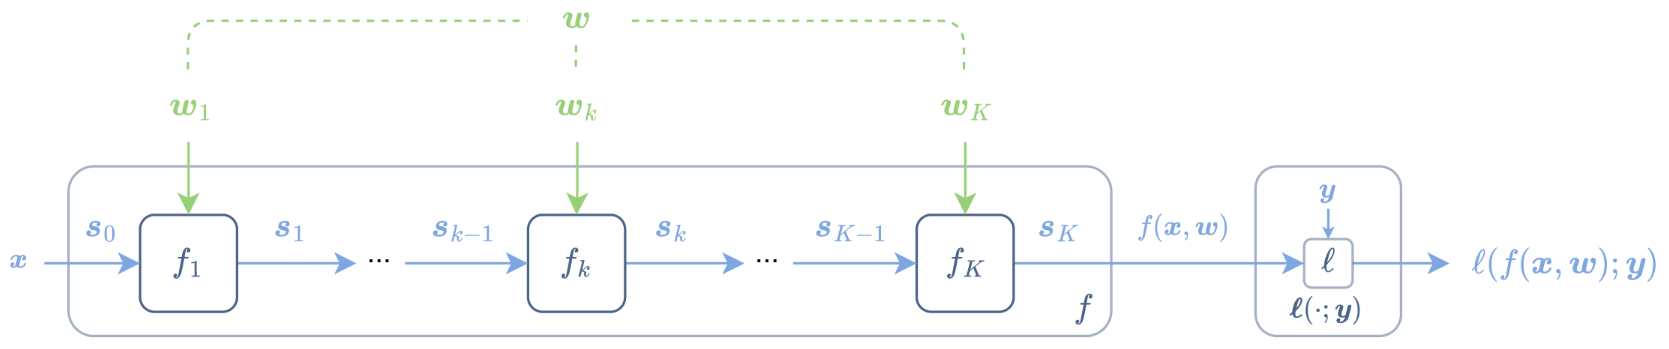
\includegraphics[width=\textwidth]{img/nn_fd.png}
    \caption{Neural network forward pass}
    \label{fig:nn_fd}
\end{figure}
And the backward pass can be represented like this:\\
\begin{figure}[H]
    \centering
    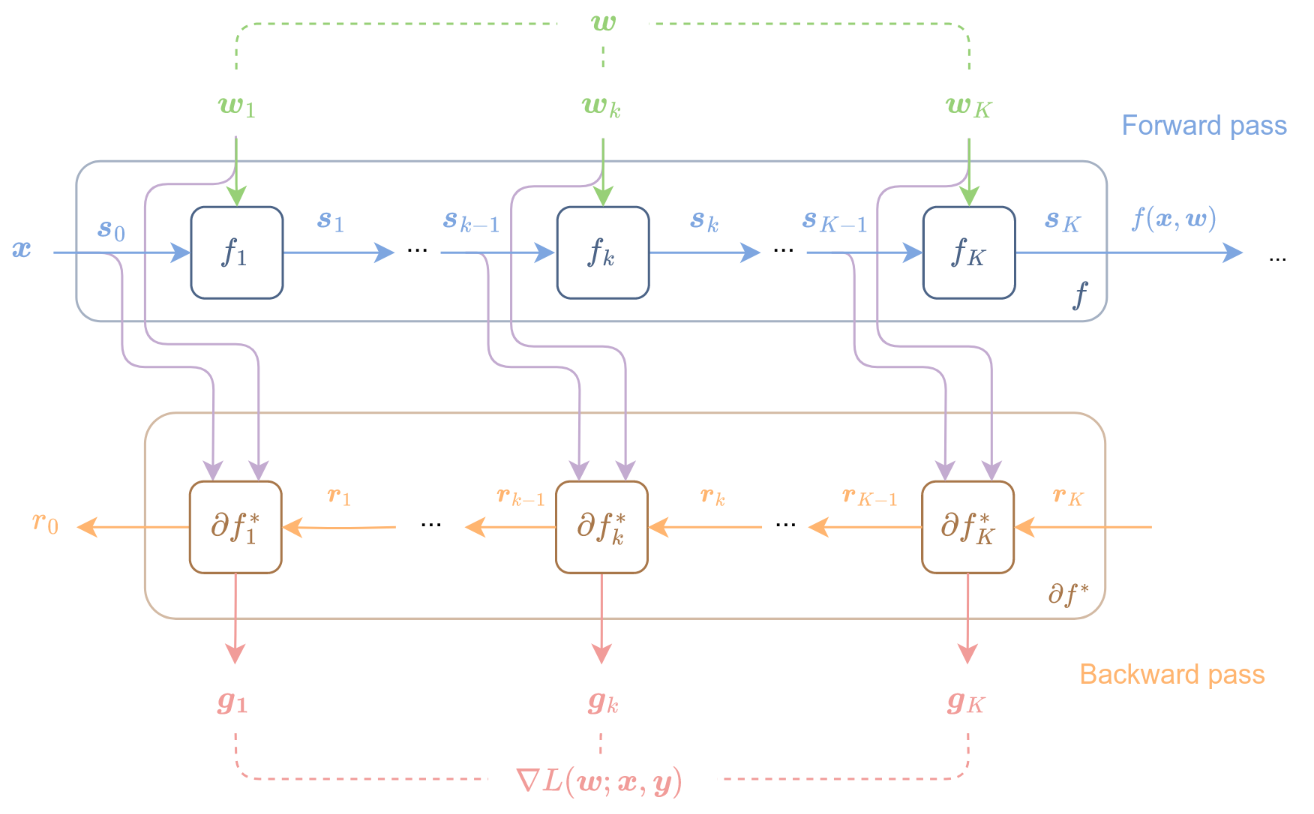
\includegraphics[width=\textwidth]{img/nn_bd.png}
    \caption{Neural network backward pass}
    \label{fig:nn_bd}
\end{figure}
\end{document}